\documentclass[3p, authoryear, review]{elsarticle} %review=doublespace preprint=single 5p=2 column
%%% Begin My package additions %%%%%%%%%%%%%%%%%%%
\usepackage[hyphens]{url}

  \journal{Submitted to Journal} % Sets Journal name


\usepackage{lineno} % add
\providecommand{\tightlist}{%
  \setlength{\itemsep}{0pt}\setlength{\parskip}{0pt}}

\usepackage{graphicx}
%%%%%%%%%%%%%%%% end my additions to header

\usepackage[T1]{fontenc}
\usepackage{lmodern}
\usepackage{amssymb,amsmath}
\usepackage{ifxetex,ifluatex}
\usepackage{fixltx2e} % provides \textsubscript
% use upquote if available, for straight quotes in verbatim environments
\IfFileExists{upquote.sty}{\usepackage{upquote}}{}
\ifnum 0\ifxetex 1\fi\ifluatex 1\fi=0 % if pdftex
  \usepackage[utf8]{inputenc}
\else % if luatex or xelatex
  \usepackage{fontspec}
  \ifxetex
    \usepackage{xltxtra,xunicode}
  \fi
  \defaultfontfeatures{Mapping=tex-text,Scale=MatchLowercase}
  \newcommand{\euro}{€}
\fi
% use microtype if available
\IfFileExists{microtype.sty}{\usepackage{microtype}}{}
\usepackage{natbib}
\bibliographystyle{apalike}
\usepackage{longtable,booktabs,array}
\usepackage{calc} % for calculating minipage widths
% Correct order of tables after \paragraph or \subparagraph
\usepackage{etoolbox}
\makeatletter
\patchcmd\longtable{\par}{\if@noskipsec\mbox{}\fi\par}{}{}
\makeatother
% Allow footnotes in longtable head/foot
\IfFileExists{footnotehyper.sty}{\usepackage{footnotehyper}}{\usepackage{footnote}}
\makesavenoteenv{longtable}
\ifxetex
  \usepackage[setpagesize=false, % page size defined by xetex
              unicode=false, % unicode breaks when used with xetex
              xetex]{hyperref}
\else
  \usepackage[unicode=true]{hyperref}
\fi
\hypersetup{breaklinks=true,
            bookmarks=true,
            pdfauthor={},
            pdftitle={USTM Resiliency Sensitivity Analysis},
            colorlinks=false,
            urlcolor=blue,
            linkcolor=magenta,
            pdfborder={0 0 0}}
\urlstyle{same}  % don't use monospace font for urls

\setcounter{secnumdepth}{5}
% Pandoc toggle for numbering sections (defaults to be off)

% Pandoc citation processing

% Pandoc header
\usepackage{booktabs}



\begin{document}
\begin{frontmatter}

  \title{USTM Resiliency Sensitivity Analysis}
    \author[Brigham Young University]{Gregory Macfarlane\corref{1}}
   \ead{gregmacfarlane@byu.edu} 
    \author[Brigham Young University]{Natalie Gray}
   \ead{nat.gray2000@gmail.com} 
      \address[Brigham Young University]{Civil and Environmental Engineering Department, 430 Engineering Building, Provo, Utah 84602}
      \cortext[1]{Corresponding Author}
  
  \begin{abstract}
  This is where the abstract should go.
  \end{abstract}
   \begin{keyword} Sensitivity Analysis Resiliency Latin Hypercube Sampling\end{keyword}
 \end{frontmatter}

\hypertarget{questions}{%
\section{Questions}\label{questions}}

There exists uncertainty in travel demand models. This is known by transportation planners but the majority do not use any particular method to quantify it. This uncertainty exists mostly due to the variance among input parameters. A coefficient of variation can be used to approximate the standard deviation of the inputs, which then provides a range of values that are possible for model input \citep{zhao2002propagation}. A sampling method can then be used to determine the possible combinations of parameter variance. Two popular sampling methods are Monte Carlo simulation and Latin Hypercube sampling. Monte Carlo simulation is capable of providing full variance probability, but requires large computations to be effective on a large scale model \citep{yang2013sensitivity}. Latin Hypercube sampling reduces the amount variants needed, but the question arises on if the same result be achieved with fewer samples, and how many samples is that?

The research questions are therefore:

\begin{itemize}
\tightlist
\item
  How many iterations of Latin Hypercube Sampling in a travel demand model are necessary to approximate random sampling methods (e.g., Monte Carlo simulation)?
\item
  Does this method of sampling have few enough iterations for statewide model application?
\end{itemize}

\hypertarget{methods}{%
\section{Methods}\label{methods}}

To examine the effects of parameter input sensitivity, a 25 zone dummy model was created using data from \url{https://github.com/ActivitySim/activitysim}, and coefficient values from the USTM Resiliency Model.

The inputs for sampling that will be used are mode choice coefficients, mode choice constants, and destination choice parameters. These inputs are shown in Table \ref{tab:MCcoeff}, and Table \ref{tab:MCconst}.

\begin{table}

\caption{\label{tab:MCcoeff}Mode Choice Coefficients}
\centering
\begin{tabular}[t]{l|r|r|r}
\hline
Name & HBW & HBO & NHB\\
\hline
CIVTT & -0.0450 & -0.0350 & -0.0400\\
\hline
CCOST & -0.0016 & -0.0016 & -0.0016\\
\hline
CWALK1 & -0.0900 & -0.0700 & -0.0800\\
\hline
AUTOCOST & 18.3000 & 18.3000 & 18.3000\\
\hline
\end{tabular}
\end{table}

\begin{table}

\caption{\label{tab:MCconst}Mode Choice Constants}
\centering
\begin{tabular}[t]{l|r|r|r}
\hline
Name & HBW & HBO & NHB\\
\hline
K\_TRN & -0.5140 & -0.9853 & -1.3020\\
\hline
K\_NMOT & 1.7602 & 0.5448 & -0.5359\\
\hline
\end{tabular}
\end{table}

The shapefile for the dummy model is shown in Figure \ref{fig:TAZmap}.

\begin{figure}

{\centering 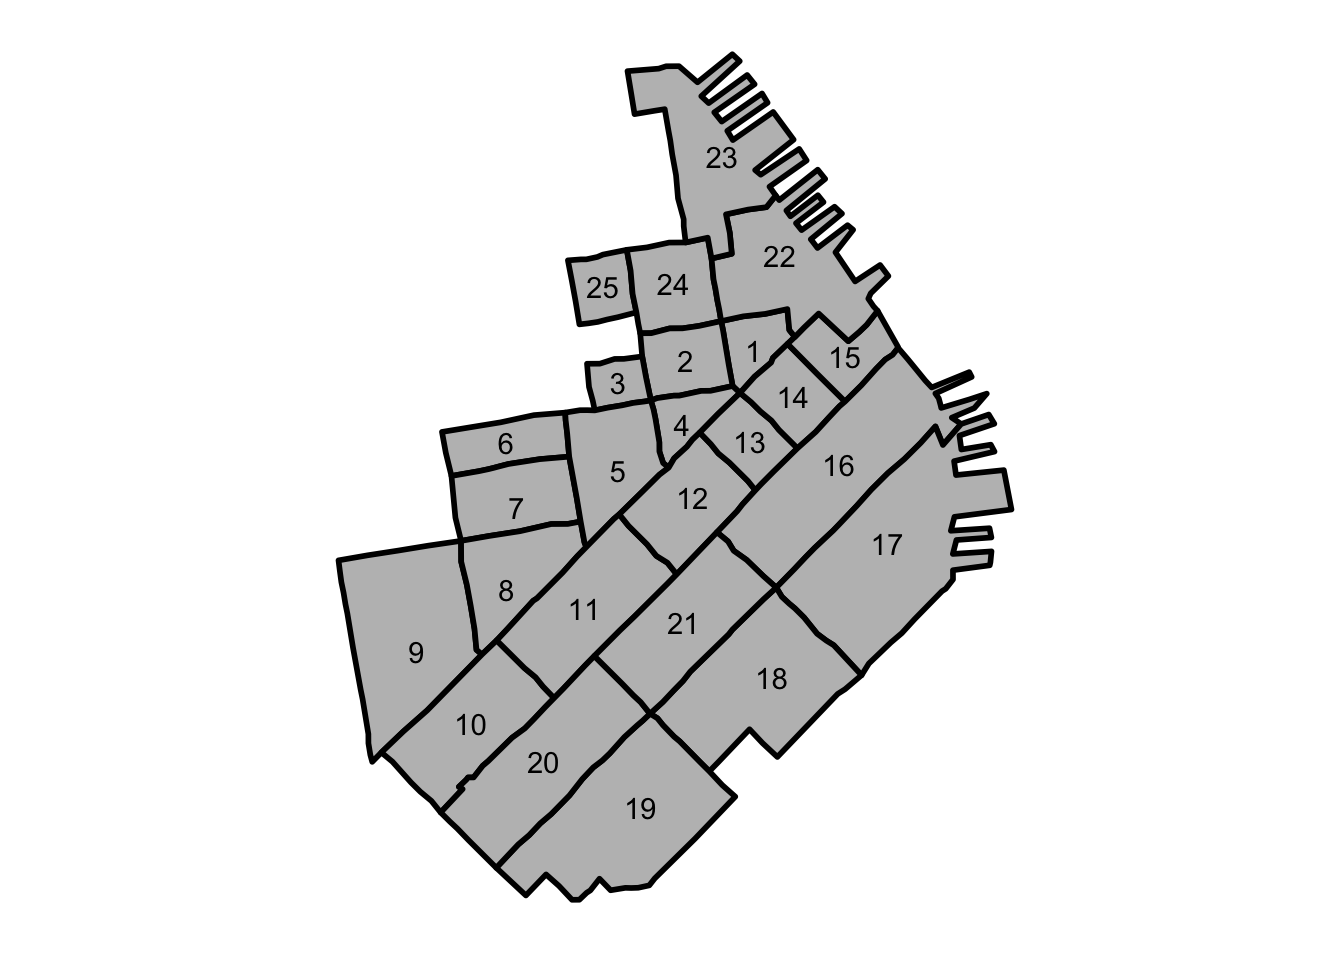
\includegraphics{ustm_resiliency_sensitivity_files/figure-latex/TAZmap-1} 

}

\caption{TAZ Map with ID}\label{fig:TAZmap}
\end{figure}

A mode choice model was created with utility equations for Home Based Work Trips(HBW), Home Based Other Trips(HBO), and Non Home Based Trips(NHB).

A coefficient of variation is used for each input parameter to determine a range for the values that can be used within the model, to estimate the sensitivity of these parameters.

The initial model was run, the change was calculated on a random selection basis, and then using latin hyoercube sampling, to see if latin hypercube sampling can estimate uncertainty in fewer runs.

\hypertarget{findings}{%
\section{Findings}\label{findings}}

Which describes the results of what you found.

\bibliography{book.bib}


\end{document}
